%%%%%%%%%%%%%%%%%%%%%%%%%%%%%%%%%%%%%%%%%
% Short Sectioned Assignment
% LaTeX Template
% Version 1.0 (5/5/12)
%
% This template has been downloaded from:
% http://www.LaTeXTemplates.com
%
% Original author:
% Frits Wenneker (http://www.howtotex.com)
%
% License:
% CC BY-NC-SA 3.0 (http://creativecommons.org/licenses/by-nc-sa/3.0/)
%
%%%%%%%%%%%%%%%%%%%%%%%%%%%%%%%%%%%%%%%%%

%----------------------------------------------------------------------------------------
%	PACKAGES AND OTHER DOCUMENT CONFIGURATIONS
%----------------------------------------------------------------------------------------

\documentclass[paper=a4, fontsize=11pt]{scrartcl} % A4 paper and 11pt font size
\usepackage{graphicx}
\usepackage[T1]{fontenc} % Use 8-bit encoding that has 256 glyphs
\usepackage{fourier} % Use the Adobe Utopia font for the document - comment this line to return to the LaTeX default
\usepackage[english]{babel} % English language/hyphenation
\usepackage{amsmath,amsfonts,amsthm} % Math packages
\usepackage{color} % This is used for highlighting text whenever you need to come back to something
%\usepackage{sectsty} % Allows customizing section commands
%\allsectionsfont{\centering \normalfont\scshape} % Make all sections centered, the default font and small caps
%\usepackage{fancyhdr} % Custom headers and footers
%\pagestyle{fancyplain} % Makes all pages in the document conform to the custom headers and footers
%\fancyhead{} % No page header - if you want one, create it in the same way as the footers below
%\fancyfoot[L]{} % Empty left footer
%\fancyfoot[C]{} % Empty center footer
%\fancyfoot[R]{\thepage} % Page numbering for right footer
%\renewcommand{\headrulewidth}{0pt} % Remove header underlines
%\renewcommand{\footrulewidth}{0pt} % Remove footer underlines
%\setlength{\headheight}{13.6pt} % Customize the height of the header

%numberwithin{equation}{section} % Number equations within sections (i.e. 1.1, 1.2, 2.1, 2.2 instead of 1, 2, 3, 4)
%\numberwithin{figure}{section} % Number figures within sections (i.e. 1.1, 1.2, 2.1, 2.2 instead of 1, 2, 3, 4)
%\numberwithin{table}{section} % Number tables within sections (i.e. 1.1, 1.2, 2.1, 2.2 instead of 1, 2, 3, 4)

%\setlength\parindent{0pt} % Removes all indentation from paragraphs - comment this line for an assignment with lots of text

%----------------------------------------------------------------------------------------
%	TITLE SECTION
%----------------------------------------------------------------------------------------

\newcommand{\horrule}[1]{\rule{\linewidth}{#1}} % Create horizontal rule command with 1 argument of height

\title{	
\normalfont \normalsize 
\textsc{Columbia University -- CUNY} \\ [25pt] % Your university, school and/or department name(s)
\horrule{0.5pt} \\[0.4cm] % Thin top horizontal rule
\huge Homework 2 - NLP/ML/Web \\ % The assignment title
\horrule{2pt} \\[0.5cm] % Thick bottom horizontal rule
}

\author{Jessica Ouyang and Joe Ellis} % Your name

\date{\normalsize\today} % Today's date or a custom date

\begin{document}

\maketitle % Print the title

%---
% Task 
%---

\section{Task -- Language Modeling}
\paragraph{}
In this problem we are tasked with attempting to modeling a language example of at least 100,000 words and another language model that is created using a seperate corpus of at least 50,000 words.  For this experiment we chose to use two famous novels as our language examples, one being ``The Scarlet Letter'' by Nathaniel Hawthorne and the other being ``A Tale of Two Cities'' written by Charles Dickens.  Both were modeled using different n-gram language models.  We also applied Laplacian smoothing and back-off to our models to create more accuracte language models.  Finally, we created a combined model trained off of both language examples.

\section{Experiments and Results}
\subsection{Task 1 -- Domain A}


\paragraph{1a -- Download Language Text}
For our first domain we chose to download and use the famous novel ``A Tale of Two Cities'' by Charles Dickens.  The novel had much more than 100,000 words.  For our train and test split we decided that we would use 60\% of the available data for test, 20\% for development, and 20\% for evalauation.

\paragraph{1b - Find N for Language Model}
After this we had to find the N for the N gram model that would be utilized for this text.  The best result in our examples for the proper N-gram model was the tri-gram model.  This first example we did not do any smoothing, therefore we evaluated only on the seen grams from the development set, and chose N that provided the lowest perplexity.  Average Perplexity per gram was calculated using the formula,

\begin{align}
Perplexity_{ave}(text) = 2^{-\frac{1}{N}\sum_1^N p(w_i)log(p(w_i))}
\end{align}

We chose to use this formula, so that different models with differing data sizes can be compared $x$.
We chose tri-gram as the best model, and the graph of the results can be seen in Figure ~ref{fig:figure1}.  The results on the test set for seen grams is $Perplexity(test)=15.426$

\begin{figure}
\centering
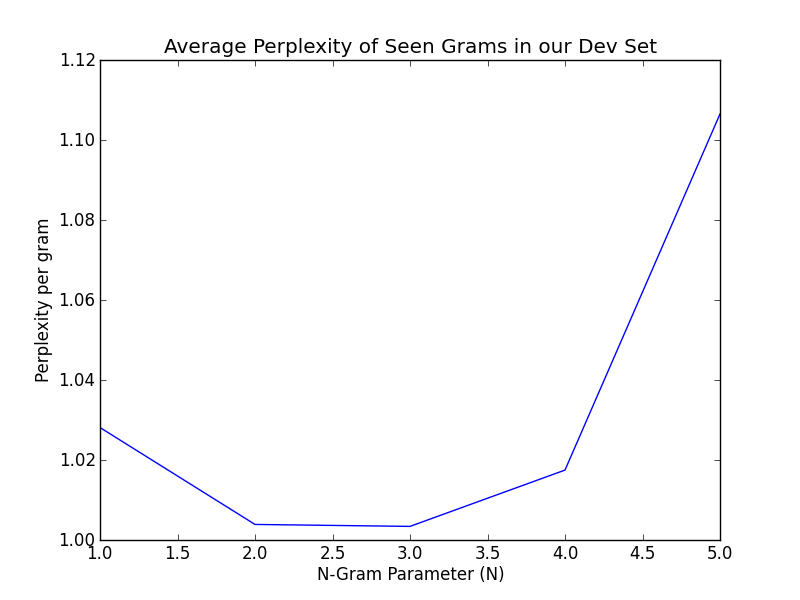
\includegraphics[scale=0.4]{figure_1.png}
\caption{N-Gram Performance for Domain A}
\label{fig:figure1}
\end{figure}

\paragraph{1c -- Laplace Smoothing}
We also utilized Laplace smoothing to solve for the best value of N with Laplace Smoothing utilized.  When we use Laplace smoothing instead of using simply $p(w)=\frac{N(w)}{N}$, we include and extra value of $V$ into the equation where $V$ is the number of distinct N-grams present.  Therefore, the new $p(w) = \frac{N(w)+1}{N+V}$.  This allows us to classify all of the values seen, but gives small probablities to unseen before grams.  The results of this modeling scheme can be seen below, and for this model tri-gram also wins out.  
However, since many of the n-grams are unseen for $n=4$ or $n=5$, the penalty is not as high as before.  The results are shown in Figure ~\ref{fig:figure2}.  
The result on the test set for all grams with smoothing is,  $Perplexity(test)=2^{31.25}$, and the total entropy is $-31.250$.

\begin{figure}
\centering
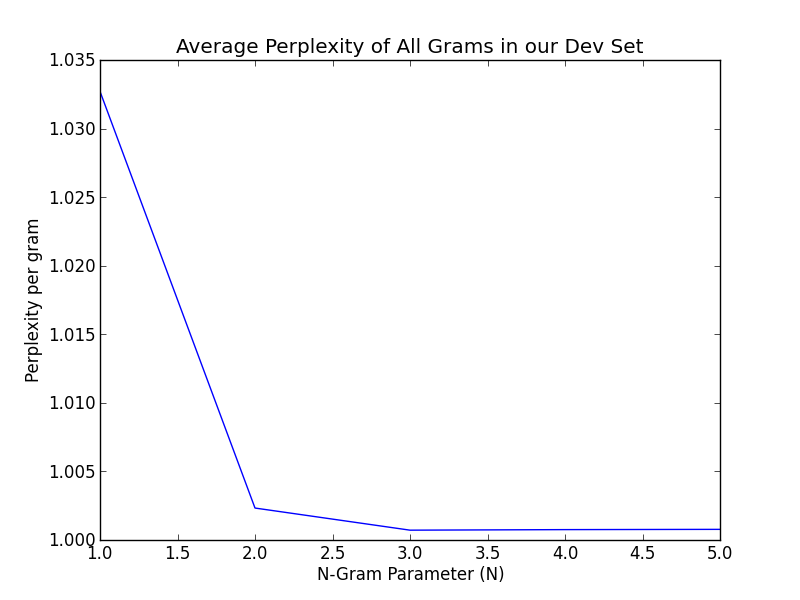
\includegraphics[scale=0.4]{figure_2.png}
\caption{N-Gram Performance for Domain A}
\label{fig:figure2}
\end{figure}

\paragraph{1d -- Back-Off}
Finally, we addressed the issue of unseen grams during training using the Back-Off parameters.  For, Back-Off we use $p(w)$ as a linear interpolation of the values of each condition probablity that makes up $p(w)$.  Therefore, the equation for back-off is as follows,

\begin{align}
p(w)=\lambda_0p(w_0) + \lambda_1p(w_1|w_0) + \lambda_2p(w_2|w_1,w_0).
\end{align}

We would have used 4-gram for back-off training, however once I got to 4-gram language representation 98\% of my grams were unseen.  
So most of the values would be unseen for this case, and therefore we chose to only perform back-off from 3.
We attempted to use a variety of different lambdas for the language model and the results can be seen below in Table ~ref{tab:table1}.  We have chosen our $\lambda$ wieghting scheme as $\lambda=(0.0,0.3,0.7)$, and this is because we wanted all $\lambda$s to be non-zero, but the unigram model was not useful for this problem. The perplexity score on our test dataset using these parameters was $Perplexity(test) = 2^{241.31}$.  

\begin{table}
\centering
\label{tab:table1}
\caption{lambda values and perplexity scores}
\begin{tabular}{|c|c|c|c|}
\hline
$\lambda_0$ & $\lambda_1$ & $\lambda_2$ & $Perplexity_{ave}(dev)$ \\ \hline \hline
0 & 0.5 & 0.5 & 1.0075  \\ \hline
0.33 & 0.33 & 0.33 & 1.0181 \\ \hline
0.2 & 0.4 & 0.4 & 1.0145 \\ \hline
0.5 & 0.25 & 0.25 & 1.0223 \\ \hline
0.25 & 0.5 & 0.25 & 1.0171 \\ \hline
0.25 & 0.25 & 0.5 & 1.0148 \\ \hline
0.1 & 0.2 & 0.7 & 1.0089 \\ \hline
0.0 & 0.3 & 0.7 & 1.0055 \\ \hline
\end{tabular}
\end{table}

\subsection{Task 2}
\paragraph{2a - Download another Domain}
For our second domain, we utilized the famous novel ``The Scarlet Letter'' by Nathaniel Hawthorne.  This book contains over 50,000 words and the train and test split of the data was the same as was used above.

\paragraph{2b - Find Optimal Language Model}
The same tests were used as those described above to find the optimal language model for this text, and we received similar results.  Once again the highest performing model was the tri-gram model with smoothing.  This model appears to work well on many datasets, however it would be useful to have more training data as many of the grams remain unseen even in this model.  The perplexity of this model on the test-set on the seen grams is $Perplexity(test)=2^{0.2627}=1.2033$.  When we utilized the $\lambda=(0.0,0.6,0.4)$ parameters and performed back-off ad smoothing on the set we received a perplexity score on our dataset of $Perplexity(test)=2^{113.5347}$

\paragraph{2c-Cross Domain Analysis}
We also attempted to see how our first domain model, the model that was trained on Dickens performed on The Scarlet Letter.  The performance was similar but slightly degraded, and the resulting average entropy per n-gram is $-0.0120$, which over the 18,652 trigrams testsed gives us  a perplexity of, $Perplexity(crossdomain) = 2^{108.0305}$.

\paragraph{2d- Interpolated Model}
Finally, we also tested on the The Scarlet Letter an interpolated model, that allowed for us to utilized both trained models for modeling.  For this model we linearly combined the probablilty received from both models using $\lambda$ parameters and the results on the development set can be seen below for multiple $\lambda$.  We have $\lambda_0$ corresponding to ``A Tale of Two Cities'' trained model and $\lambda_1$ corresponds to ``The Scarlet Letter'' trained model.  
These values outperform just the Scarlet Letter Model by itself on the test data, greatly.

\begin{table}
\centering
\label{tab:table2}
\caption{lambda values and perplexity scores for linearly combined model}
\begin{tabular}{|c|c|c|}
\hline
$\lambda_0$ & $\lambda_1$ & $Perplexity(dev)$ \\ \hline \hline
0.5 & 0.5 & $2^{88.62}$ \\ \hline
0.2 & 0.8 & $2^{84.42}$ \\ \hline
0.3 & 0.7 & $2^{85.88}$ \\ \hline
\end{tabular}
\end{table}

\paragraph{2e - Interpolated Model Performance}
The testing was performed on the ``The Scarlet Letter'' test set, and the resulting perplexity using interpolation parameters $(\lambda_{int} = (0.2,0.7)$ is $Perplexity(test) = 2^{77.39}$.  This shows just how useful it is to have multiple models and broaden our training data.  The interpolated model outperforms both singluar models by itself.

\section{Linguistic Oriented Section}

Pereira argues that formal grammar and statistical estimation are not as irreconcilable as they were once thought to be.  Not only are computational approaches functionally successful in natural language processing tasks, but they are becoming more acceptable to linguists.

Opponents of the information theoretic approach to linguistics have argued purely statistical learning would leave humans unable to process strings that had never been encountered before.  Since no one could possibly experience all grammatical strings, and yet humans are able to parse new strings just fine, this must mean that language acquisition must not be based on statistics but rather on some innate sensitivity to Universal Grammar.  However, this argument assumes that all statistical learning overfits the training data, which is not true.  The success of a machine learning algorithm depends on its ability to generalize to new, previously unseen inputs, and there is no reason why a statistical language model in a human brain should be any different.  

However, I do not think it is plausible for humans to learn language the same way a computer does.  Most humans are not comfortable with probabilities -- this is clear not only from such problems as the birthday "paradox" and the Monty Hall problem, but from all the wailing and gnashing of teeth that goes on in a randomized algorithms of machine learning class.  Even statistically-trained human brains can not handle the tremendous amounts of data that computers can, so it is unlikely that humans process language using the same statistical models that computers do.  It is possible that a human might be able to do sophisticated statistical modeling subconsciously, but I find it doubtful (although the ability of German speakers to keep track of their verbs is very impressive, so who knows).  I think that the right conclusion to draw from this argument is that there is no reason why humans cannot extrapolate from previously seen language -- in fact, humans are sometimes a little too good at generalization (the availability heuristic)!  The two views of language acquisition need not be in conflict; why not have Universal Grammar as a set of priors instead of a hard-and-fast set of rules?

Pereira also shows that some of the arguments against statistical methods were based on older, less sophisticated models.  No one would argue, for instance, that the Markov assumption accurately models a human's mental state when processing language, even if it often works well enough in practice.  However, conditional random fields address this particular weakness by accounting for greater distances between dependent variables in a sequence, both hidden and observed.  Again, I think that conflating machine learning techniques with human language processing is a mistake.  While the use of statistical inference in human language processing is plausible, I doubt even its proponents would claim that all humans walk around with fully-trained CRFs in their heads.  

The question of tractability goes in both directions.  Just as a human cannot do complex statistical modeling in his head, so a machine learning technique is subject to concerns of running time and space.  An algorithm must run reasonably quickly and not use too much memory -- the Markov assumption is used for precisely this reason.  It is not that computational linguists are trying to assert that formal linguistics is wrong.  Despite Fred Jelinek's famous claim that "Every time I fire a linguist, the performance of the speech recognizer goes up," linguistically-motivated features are in use.  Work on discourse relations, for example, depends heavily on syntactic features, from part-of-speech tags to partial trees.  However, the syntactic theories that formal linguists use are too complex to use in computational linguistics.  Even if computational linguists wanted to stay true to current theories in formal linguistics, it would be an impossible task.  

Formal linguists do not agree even amongst themselves on just what Universal Grammar is.  How do we deal with Irish word order?  Do we allow ternary-branching for conjunctions, or do we resign ourselves to an unequal relationship where one conjunct is the head and the other is the complement?  Statistical parsers need an agreed-upon set of rules, and formal linguistics is unable to provide one.  In addition, linguists posit a good deal of movement in order to account for surface word order.  Verbs raise and lower, wh-words leap to the top of the tree, and all the while, case-checking is making sure no one goes where they should not go.  This is a lot for a computer to handle, and machine learning algorithms do pretty well without this extra information.  The choice not to precisely follow current formal linguistic theories is not made because computational linguists mistrust the work of formal linguists, but that to do so would require a tremendous amount of work for not a lot of expected performance gains.  

Pereira rebuts the argument that the stimulus of observed language is too impoverished for a child to learn by comparing it to semi- or distantly-supervised learning.  First, I do not believe the claim that children receive no negative examples at all.  There are, of course, cases of speaker error, where an adult misspeaks and corrects himself in front of the child.  As semi-supervised learning techniques show, a very small seed of examples can be sufficient for learning.  But there has also been work on semi-supervised learning with a seed containing only positive examples.  This approach avoids having to hand-annotate negative training examples and allows the classifier to label slices of the data with positive and negative labels itself as it trains.  Analogously, we have a child who is presented with many positive examples by adults.  The child can generates candidate sentences in his head, some of which he may label as ungrammatical, and these serve as his negative examples for the next round of learning.  

Another counterargument would be that bilingual children are frequently exposed to negative examples.  My parents' English is very good overall, but they make some systematic errors due to the differences between English and Mandarin grammars.  For example, my mother always moves wh- words, even when it is not necessary.  There is no wh- movement in Mandarin, but there is in English, and she has over-generalized the wh-movement rules (further evidence that humans can generalize!).  She produces sentences such as "I don't know what is that" instead of "I don't know what that is."  A child growing up with parents who are not native English speakers will hear many ungrammatical English sentences.  If he recognizes that the English he hears at school is more likely to be correct, and the English at home is more likely to be incorrect, he will have what amounts to some noisily-labeled negative examples in the English he hears at home. 

\end{document}